% to-do:
% ------
% - merge in population results
% - discuss limitations of everything we are doing

\documentclass[pdftex]{beamer}
%\input{vc}

% set paper size
% 1.77778 is the ratio of 16 to 9
\setlength{\paperheight}{2.75in} % going small!
\setlength{\paperwidth}{1.77778\paperheight}
% 1.33333 is the ratio of 4 to 3
%\setlength{\paperheight}{3.0in} % way small!
%\setlength{\paperwidth}{1.33333\paperheight}

% set lengths given paper
\setlength{\textheight}{0.95\paperheight}
\setlength{\textwidth}{0.85\paperwidth}

% import the next thing *after* the lengths and sizes
\usepackage{amssymb,amsmath,mathrsfs}
\usecolortheme{default}

% this one is debatable
\renewcommand{\emph}[1]{\textbf{#1}}

%%% color commands
\newcommand{\whiteonblack}{%
  \colorlet{fg}{white}
  \colorlet{bg}{black}
  \setbeamercolor{normal_text}{fg=white,bg=black}
  \setbeamercolor{background canvas}{fg=white,bg=black}
  \setbeamercolor{alerted_text}{fg=yellow}
  \setbeamercolor{example_text}{fg=white}
  \setbeamercolor{structure}{fg=white}
  \setbeamercolor{palette_quaternary}{fg=white}
}
\newcommand{\blackonwhite}{%
  \colorlet{fg}{black}
  \colorlet{bg}{white}
  \setbeamercolor{normal_text}{fg=black,bg=white}
  \setbeamercolor{background canvas}{fg=black,bg=white}
  \setbeamercolor{alerted_text}{fg=blue}
  \setbeamercolor{example_text}{fg=black}
  \setbeamercolor{structure}{fg=black}
  \setbeamercolor{palette_quaternary}{fg=black}
}
\xdefinecolor{pink}{rgb}{1.0,0.9,0.9}

%%% size and shape commands
\newlength{\figurewidth}
\setlength{\figurewidth}{\textwidth}
\newlength{\figureheight}
\setlength{\figureheight}{0.9\textheight}

%%% text commands
\newcommand{\project}[1]{\textsl{#1}}
  \newcommand{\tc}{\project{The~Cannon}}
  \newcommand{\an}{\project{Astrometry.net}}
  \newcommand{\euclid}{\project{Euclid}}
  \newcommand{\flickr}{\project{flickr}}
  \newcommand{\gaia}{\project{Gaia}}
  \newcommand{\galex}{\project{GALEX}}
  \newcommand{\kepler}{\project{Kepler}}
  \newcommand{\GALEX}{\galex}
  \newcommand{\hst}{\project{HST}}
  \newcommand{\hipparcos}{\project{Hipparcos}}
  \newcommand{\lsst}{\project{LSST}}
  \newcommand{\sdss}{\project{SDSS}}
  \newcommand{\sdssiii}{\project{SDSS-III}}
  \newcommand{\sdssiv}{\project{SDSS-IV}}
  \newcommand{\boss}{\project{BOSS}}
  \newcommand{\apogee}{\project{APOGEE}}
  \newcommand{\osss}{\project{OSSS}}
  \newcommand{\ska}{\project{SKA}}
  \newcommand{\vo}{\project{VO}}
  \newcommand{\rttd}{\project{Right Thing To Do}$^{\mbox{\scriptsize\sffamily{TM}}}$}
\newcommand{\foreign}[1]{\textit{#1}}
\newcommand{\latin}[1]{\foreign{#1}}
  \newcommand{\cf}{\latin{cf.}}
  \newcommand{\eg}{\latin{e.g.}}
  \newcommand{\etal}{\latin{et~al.}}
  \newcommand{\etc}{\latin{etc.}}
  \newcommand{\ie}{\latin{i.e.}}
  \newcommand{\vs}{\latin{vs.}}

%%% math-mode commands
\newcommand{\unit}[1]{\mathrm{#1}}
  \newcommand{\rad}{\unit{rad}}
  \newcommand{\s}{\unit{s}}
  \newcommand{\yr}{\unit{yr}}
  \newcommand{\km}{\unit{km}}
  \newcommand{\kmps}{\km\,\s^{-1}}
\newcommand{\mmatrix}[1]{\boldsymbol{#1}}
\newcommand{\tv}[1]{\boldsymbol{#1}}
\newcommand{\dd}{\mathrm{d}}
\newcommand{\given}{\,|\,}
\newcommand{\transpose}[1]{{#1}^{\mathsf{\!T}}}
\DeclareMathOperator*{\diag}{diag}
 % hogg standard colors

\title{How rare are Earths? \\ And how common are Jupiters?}
\author[David W. Hogg (NYU)]{David W. Hogg \textsl{(NYU \& MPIA \& Simons)}\\[1ex]
  \textsl{\footnotesize
    in collaboration with:
    Dan~Foreman-Mackey~\textsl{(UW)},
    Bernhard~Sch\"olkopf~\textsl{(MPI-IS)},
    Dun~Wang~\textsl{(NYU)}}}
\date{D. E. Shaw / 2017 March 2}

\newcommand{\conclusions}{%
\begin{frame}
  \frametitle{Summary}
  \begin{itemize}
  \item Planets are abundant around other stars but exceedingly hard to detect.
    \begin{itemize}
    \item 1 to 50 percent of Sun-like stars host Earths
    \item long-period Jupiters and Saturns might be \emph{very} common
    \end{itemize}
  \item \emph{Search} involves extracting tiny, sparse signals from noisy data.
    \begin{itemize}
    \item both stellar and spacecraft-induced noise
    \item \emph{engineering improvements have huge impact}
    \end{itemize}
  \item \emph{Population inferences} require expensive noise propagation.
    \begin{itemize}
    \item hierarchical modeling
    \end{itemize}
  \end{itemize}
\end{frame}}

\begin{document}

\begin{frame}
  \titlepage
\end{frame}

\conclusions

\begin{frame}
  \frametitle{The NASA \kepler\ and K2 Missions}
  \begin{itemize}
  \item Stared at $1.5\times 10^5$ stars for 4 years\ldots
    \begin{itemize}
    \item $7\times 10^4$ measurements per star
    \item all data completely public
    \end{itemize}
  \item \ldots plus another $10^6$ (ish) for $80$ days (ish)
  \item Looking for planet \emph{transit signals}
  \item Found \emph{thousands of planets around other stars}
  \end{itemize}
\end{frame}

\begin{frame}
  \frametitle{The NASA \kepler\ and K2 Missions}
  ~\hfill
  \includegraphics<1>[height=\figureheight]{kepler/750603main_Ball_Kepler_A8468_275_lg_blog_main_horizontal.jpg}
  \includegraphics<2>[height=\figureheight]{kepler/Kepler_FOV_hiRes.jpg}
  \includegraphics<3>[height=\figureheight]{kepler/FirstLightLogInvertedPink_wslbld2400.jpg}
  \includegraphics<4>[height=\figureheight]{1502.04715/figures-de-trended.pdf}
  \includegraphics<5>[height=\figureheight]{1502.04715/figures-folded.pdf}
  \includegraphics<6>[height=\figureheight]{dfm/full_sample.pdf}
\end{frame}

\begin{frame}
  \frametitle{Exoplanet populations}
  ~\hfill
  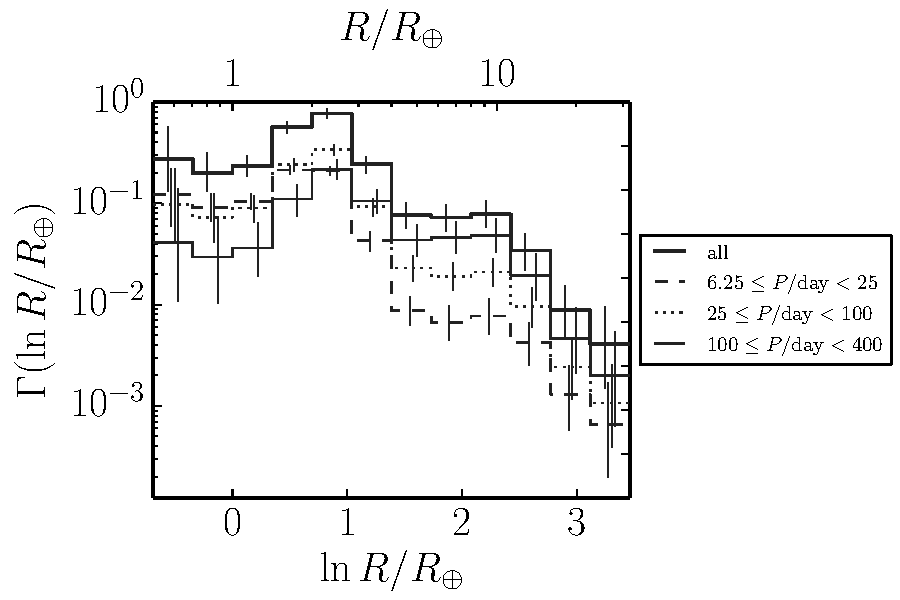
\includegraphics[height=\figureheight]{1406.3020/results-radius.pdf}
\end{frame}



\begin{frame}
  \frametitle{Earth-like transit signals}
  \begin{itemize}
  \item requires good alignment (percent-level)
  \item Earth blocks $10^{-4}$ of the light from the Sun
  \item it does this for 13 hours out of every 365.25 days
  \item the Sun has stochastic variability with an amplitude larger than the signal
  \end{itemize}
\end{frame}

%% Syntactical

\begin{frame}
  \frametitle{Search: assumptions}
  \begin{itemize}
  \item There are three sources of noise:
    \begin{itemize}
    \item shot noise, spacecraft variability, stellar variability
    \end{itemize}
  \item These can be treated as additive and Gaussian.
    \begin{itemize}
    \item differ only in their covariance properties
    \end{itemize}
  \item We know what a planet transit looks like.
    \begin{itemize}
    \item it enters the model as the mean function of the Gaussian process
    \end{itemize}
  \end{itemize}
\end{frame}

\begin{frame}
  \frametitle{Search: assumptions}
  \begin{itemize}
  \item $-2\,\ln L = \transpose{[y - m]}\cdot V^{-1}\cdot [y - m] + \ln\det V$
  \item $y$ is your data, $m$ is your model (of a planet signal!).
  \item $V$ encodes your beliefs about your (Gaussian) noise.
  \end{itemize}
\end{frame}

\begin{frame}
  \frametitle{Systematic noise {\footnotesize (Foreman-Mackey \etal, 1502.04715)}}
  ~\hfill
  \includegraphics<1>[trim=100 100 100 100, clip, height=\figureheight]{brownbag/brownbagp10.pdf}
  \includegraphics<2>[trim=100 100 100 100, clip, height=\figureheight]{brownbag/brownbagp14.pdf}
\end{frame}

\begin{frame}
  \frametitle{Causal idea}
  \begin{itemize}
  \item If a star's behavior can be predicted confidently by
    other stars, then that behavior must be being imprinted by
    the spacecraft.
  \item We are using these ideas to separate spacecraft-induced from
    intrinsic stellar variability {\footnotesize (Wang \etal, arXiv:1508.01853;
    Sch\"olkopf \etal, arXiv:1505.03036)}.
  \end{itemize}
\end{frame}

\begin{frame}
  \frametitle{Systematic noise model}
  \begin{itemize}
  \item Imagine that we believe that the spacecraft noise
    can be modeled as a sum of $M$ basis vectors.
  \item If we can put a Gaussian prior on the linear amplitudes, we
    can fully represent this noise by adding in a rank-$M$ covariance
    matrix.
  \item This is equivalent to fitting and marginalizing!
  \end{itemize}
\end{frame}

\begin{frame}
  \frametitle{Systematic noise model}
  \begin{eqnarray}
    -2\,\ln L &=& \transpose{[y - m]}\cdot V^{-1}\cdot [y - m] + \ln\det V
    \nonumber \\
    V &=& C + B\cdot\Lambda\cdot\transpose{B}
    \nonumber \\
    C &=& \mbox{diagonal photon-noise variance}
    \nonumber \\
    B &=& \mbox{block of $M$ basis vectors}
    \nonumber \\
    \Lambda &=& \mbox{$M\times M$ prior variance; can $\rightarrow\infty$}
    \nonumber
  \end{eqnarray}
\end{frame}

\begin{frame}
  \frametitle{Systematic noise model}
  \begin{itemize}
  \item $y$ is your data, $m$ is your model of the planet signal.
  \item $C + B\cdot\Lambda\cdot\transpose{B}$ encodes your beliefs
    about your (Gaussian) noise, which now has a systematics
    component.
    \begin{itemize}
    \item (non-stationary Gaussian process)
    \end{itemize}
  \end{itemize}
\end{frame}

\begin{frame}
  \frametitle{Systematic noise {\footnotesize (Foreman-Mackey \etal, 1502.04715)}}
  ~\hfill
  \includegraphics<1>[trim=100 100 100 100, clip, height=\figureheight]{brownbag/brownbagp10.pdf}
  \includegraphics<2>[trim=100 100 100 100, clip, height=\figureheight]{brownbag/brownbagp14.pdf}
  \includegraphics<3>[trim=100 100 100 100, clip, height=\figureheight]{brownbag/brownbagp15.pdf}
  \includegraphics<4>[trim=100 100 100 100, clip, height=\figureheight]{brownbag/brownbagp17.pdf}
  \includegraphics<5>[trim=100 100 100 100, clip, height=\figureheight]{brownbag/brownbagp18.pdf}
\end{frame}

\begin{frame}
  \frametitle{Exoplanet discovery {\footnotesize (Foreman-Mackey \etal, 1502.04715)}}
  ~\hfill
  \includegraphics<1>[height=\figureheight]{1502.04715/figures-corr.pdf}
  \includegraphics<2>[height=\figureheight]{1502.04715/figures-linear.pdf}
  \includegraphics<3>[height=\figureheight]{1502.04715/figures-periodic.pdf}
  \includegraphics<4>[height=\figureheight]{1502.04715/figures-de-trended.pdf}
  \includegraphics<5>[height=\figureheight]{1502.04715/figures-folded.pdf}
  \includegraphics<6>[height=\figureheight]{1502.04715/figures-candidates.pdf}
\end{frame}

\begin{frame}
  \frametitle{Stellar variability noise model}
  \begin{eqnarray}
    -2\,\ln L &=& \transpose{[y - m]}\cdot V^{-1}\cdot [y - m] + \ln\det V
    \nonumber \\
    V &=& C + B\cdot\Lambda\cdot\transpose{B} + K
    \nonumber \\
    K_{ij} &=& K(|t_i - t_j|; \theta)
    \nonumber
  \end{eqnarray}
\end{frame}

\begin{frame}
  \frametitle{Implementation details}
  \begin{itemize}
  \item Brute-force search in period-phase space, computing evidence for billions of hypotheses.
  \item There are many applied-math tricks for making things much
    faster than $N^{2.6}$.
  \item Use \project{george} {\footnotesize (Foreman-Mackey \etal)}.
  \item Marginalizing out the kernel hyperparameters $\theta$ is (in
    general) very expensive.
  \end{itemize}
\end{frame}

\begin{frame}
  \frametitle{Gaussianity}
  \begin{itemize}
  \item Gaussians are magic\ldots
  \item \ldots but
    \begin{itemize}
    \item outliers are death
    \item variabilities are all skew
    \item multiplicative noise?
    \end{itemize}
  \item Generalizations are intractable or evil.
    \begin{itemize}
    \item dictionary methods, other processes
    \item the copula
    \end{itemize}
  \end{itemize}
\end{frame}

\conclusions

\begin{frame}
  \frametitle{Population inferences: assumptions}
  \begin{itemize}
  \item We are given a catalog of exoplanets with no false positives.
  \item We are also given a ``completeness'' or ``efficiency'' estimate as a function of parameters.
  \item Planets are independently drawn from some smooth, True distribution and ``noisified''.
    \begin{itemize}
    \item (``True'' $\equiv$ what would be measured with a \emph{far better experiment})
    \end{itemize}
  \item The catalog comes with proper uncertainty estimates.
    \begin{itemize}
    \item posterior samplings under an \emph{interim prior}
    \end{itemize}
  \end{itemize}
\end{frame}

\begin{frame}
  \frametitle{Exoplanet populations {\footnotesize (Foreman-Mackey \etal, arXiv:1406.3020)}}
  ~\hfill
  \includegraphics<1>[height=\figureheight]{1406.3020/results-results.pdf}
  \includegraphics<2>[height=\figureheight]{1406.3020/results-period.pdf}
  \includegraphics<3>[height=\figureheight]{1406.3020/results-radius.pdf}
  \includegraphics<4>[height=\figureheight]{1406.3020/results-rate.pdf}
  \includegraphics<5>[width=0.8\textwidth]{1406.3020/figures-comparison.pdf}
\end{frame}

\begin{frame}
  \frametitle{Long-period planets}
  \begin{itemize}
  \item If a planet has such a long orbit that it transits only once,
    the problem is much harder.
    \begin{itemize}
    \item must distinguish a single transit from a noise fluctuation
    \item better noise models needed
    \end{itemize}
  \end{itemize}
\end{frame}

\begin{frame}
  \frametitle{Population inferences: implementation notes}
  \begin{itemize}
  \item We did the low-level inference with an importance sampling.
    \begin{itemize}
    \item method pioneered by us {\footnotesize (Hogg, \etal, arXiv:1008.4146)}
    \item capitalizes on astronomers' \emph{love of samplings}
    \end{itemize}
  \item We used Elliptical Slice Sampling to perform the high-level inference.
    \begin{itemize}
    \item {\footnotesize (Murray \etal, arXiv:1001.0175)}
    \end{itemize}
  \item New input catalogs are very different.
    \begin{itemize}
    \item A lot has changed since 2014!
    \end{itemize}
  \end{itemize}
\end{frame}

\conclusions

\end{document}
